\section{Aussagenlogik}

\begin{frame}{Modelle}
	\begin{Definition}
		Sei $G$ eine aussagenlogische Formel. \\
		Eine Interpretation $I$ heißt \textbf{Modell} von $G$, wenn gilt: \quad $val_I(G) = \W$. \\
		\pause
		\medskip
		Sei $\Gamma$ eine Formelmenge.
		Eine Interpretation $I$ heißt \textbf{Modell} von $\Gamma$, wenn für alle Formeln $G \in  \Gamma$ gilt: \quad $val_I(G) = \W$.
	\end{Definition}
	\bigskip
	\pause
	\begin{block}{Schreibweisen}
		$\Gamma \models G$: jedes Modell von $\Gamma$ auch Modell von $G$ \\
		Beispiel: \quad $\set{A,B,C} \models G$ \quad Jedes Modell von $A, B$ \textbf{und} $C$ ist auch Modell von $G$ \\
		\medskip
		Schreibe $H \models G$ statt $\set{H} \models G$ \\
		\medskip
		Schreibe $\models G$ statt $\set{} \models G$ \\
		\impl G ist \emph{Tautologie} oder \emph{allgemeingültig} 
	\end{block}
\end{frame}

\begin{frame}{Modelle}
	\begin{Definition}
		Eine Formel $G$ heißt \textbf{erfüllbar}, wenn für mindestens ein $I$ wahr. \\
		
	\end{Definition}
	\pause
	\begin{Beispiel}
		Alle Modelle von \mword{(C \boder \bnot C) \bimp \left(\bnot(B \bimp A)\right)}? \\
		\pause
		\impl $I_1, I_2 \from \set{\word A, \word B, \word C} \functionto \BB, \; 
		I_1(v) = 
		\caseslr{\F, & v = \word A \\
				\W, & v = \word B \\
				\W, & v = \word C}, \;
		I_2(v) = 
		\caseslr{\F, & v = \word A \\
				\W, & v = \word B \\
				\F, & v = \word C}$. \\
		\impl Formel \emph{erfüllbar}. \\
		\pause
		\medskip
		Alle Modelle von \mword{\bnot(C \bimp C)}? \\
		\pause
		\impl Gibt keine, Formel \emph{unerfüllbar}.
	\end{Beispiel}
\end{frame}

\begin{frame}{Tautologie, Äquivalenz}
	\begin{Definition}
		Eine Formel $G$ heißt \textbf{Tautologie}, wenn für alle möglichen $I$ wahr. \\
		\pause
		\medskip
		Kurzschreibweise: Für Formeln $G$ und $H$ ist \\
		$$\bleftBr G \bgdw H \brightBr :\equiv \bleftBr\bleftBr G \bimp H \brightBr \bund \bleftBr H \bimp G\brightBr\brightBr$$ \\
		\medskip
		\alert{\textbf{Bitte aufpassen mit Pfeilen: \quad $\bgdw$ vs. $\gdw$ \quad $\bimp$ vs. $\impl$}}
	\end{Definition}
	\pause
	\begin{block}{Lemma}
		Für Formeln $G$ und $H$ gilt \\
		\[ G \equiv H \quad \text{ genau dann, wenn } \quad G \bgdw H \text{ Tautologie ist.} \]
	\end{block}
	\pause
	\begin{Beispiel}
		\centered{$\bnot\bnot G \bgdw G$ ist Tautologie, also $\bnot\bnot G \equiv G$}
	\end{Beispiel}
\end{frame}

\begin{frame}{Aussagenkalkül}
	\begin{block}{Was ist ein Kalkül?}
		\begin{itemize}
			\item Ein \emph{Rechensystem}: \; \textbf{Dinge} und was man mit ihnen \textbf{anstellen} darf. \\
			Bsp.: \quad $\R$ und $+, -, \·, /$ \qquad Schachbrett, Figuren und Zugregeln
		\end{itemize}
	\end{block}
	\pause
	\begin{block}{Aussagenkalkül}
		Haben
		\begin{itemize}
			\item Syntaktisch korrekte Formeln $For_{AL}$ \\
			\impl können erfüllbar sein oder nicht 
			\item Davon nennen wir einige bestimmte \textbf{Axiome} \\
			\impl setzen wir als Tautologien voraus
			\item Eine \emph{Schlussregel}: \textbf{Modus Ponens} \\
			...um neue Tautologien zu konstruieren
		\end{itemize}
	\end{block}
\end{frame}

\begin{frame}{Axiome, Modus Ponens}
	\begin{block}{Axiome}
		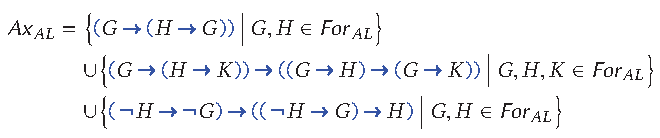
\includegraphics[width=.90\linewidth]{../figures/Axiome} \\
		Wir bestimmen: Das sind unsere „Basis-Tautologien“.
	\end{block}
	\pause
	\begin{block}{Modus Ponens (MP)}
		
		\begin{columns}[T] 
			\begin{column}[T]{.45\textwidth} 
				\vspace{-.6\baselineskip}
				\begin{itemize}
					\item<2-> Wenn $G$ gilt
					\item<2-> und $G \bimp H$ gilt \\ \mbox{}
					\implitem<2-> dann gilt auch $H$.
					\item<4-> Schreibweise: \deduction{G \qquad G \bimp H \concludes H} 
				\end{itemize}
			\end{column}
			\hspace{-2\baselineskip}
			\begin{column}[T]{.55\textwidth} 
				\vspace{-.6\baselineskip}
				\begin{itemize}
					\item<3-> Wir wissen: „Es regnet.“
					\item<3-> Wir erinnern uns: \\ „Wenn es regnet, ist die Straße nass.“
					\implitem<3-> Also wissen wir: „Die Straße ist nass“.
				\end{itemize}
				\hspace{.6\baselineskip} \only<5->{\fbox{\parbox{.9\linewidth}{Mit MP können wir aus bekannten \\ Wahrheiten neue konstruieren!}}}
			\end{column}
		\end{columns}
		
	\end{block}
\end{frame}

\begin{frame}{Ableitungen}
	Haben Formelsammlung $\Gamma$ („Hypothesen“/„Prämissen“), \\
	wollen eine Formel $G$ daraus ableiten
	\pause
	\begin{block}{Ableitung von $G$ aus $\Gamma$}
		Eine „Abfolge“ von Formeln, die in $G$ mündet \quad (Schreibweise: \; $\Gamma \vdash G$) \\
		Was dürfen wir machen?
		\pause
		\begin{itemize}
			\item<+-> aus syntaktisch korrekten Formeln \emph{Axiome} bilden und hinschreiben
			\item<.-> \emph{Prämissen} aus $\Gamma$ hinschreiben
			\item<.-> aus zwei vorherigen Formeln mit \emph{Modus Ponens} eine neue konstruieren
			\implitem<+-> das machen wir solange, bis wir $G$ konstruiert haben
		\end{itemize}
	\end{block}
\end{frame}

\begin{frame}{Beweisbarkeit}
	\begin{block}{Beweis von $G$}
		\impl Ableitung von $G$ aus $\Gamma  = \emptyset$ \\
		\impl Wir verwenden nur Axiome und MP! \\
		Schreibweise: \quad $\vdash G$ \qquad „$G$ ist beweisbar“ \\
		Ein solches beweisbares $G$ nennen wir \textbf{Theorem} des Kalküls.
	\end{block}
	\pause 
	\begin{block}{Lemma}
		Eine Formel $G$ ist genau dann Tautologie, wenn $G$ ein Theorem des Kalküls ($=$~im Kalkül beweisbar) ist. \\
		\smallskip
		\centered{--- bzw. ---} 
		\smallskip
		Für jede Formel $G$ gilt: \qquad $\models G \; \Gdw \; \vdash G$.
	\end{block}
	\pause
	\begin{block}{Lemma}
		Für Formeln $G$, $H$ gilt $G \vdash H$ genau dann, wenn $\vdash \bleftBr G \bimp H \brightBr$.
	\end{block}
\end{frame}
